% Čo by mala kapitola obsahovať
% - popísať ako sa pracuje s jednotlivými aplikáciami z pohľadu používateľa, aj screenshoty
% - popísať kritériá, tabuľka s kritériami - use casy
% - popísať slovne ako jednotlivé aplikácie spĺňajú dané kritériá 
% - tabuľka s porovnaním aplikácií vrátane mojej 
\chapter{Existing solutions}
Now that we have stated what shall the application do, we will discuss the currently available solutions which solve similar problems to our application.
In this chapter we are going to show applications and how a user can use them.
After that, we will describe criteria with which we will describe these applications and measure how the applications achieve these criteria.
Then ... a table where are all application are compared with our application.

\section{Applications with interactive menus}
For restaurant guest
We are going to look at available existing applications which are similar to our application.

\subsection{Allergy Menu}
Allergy Menu provides restaurant guests with interactive menus.
There are allergen icons in the menu item's description.
A guest can interact with the menu by choosing what allergens they want to avoid.
A guest can also select an option that they are either a vegan or vegetarian.
The application filters out items of a menu to meet the guest's preferences.
The application allows a restaurant employee create a menu and specify what allergens are contained in each item of the menu.

\begin{figure}[h]
  \centering
  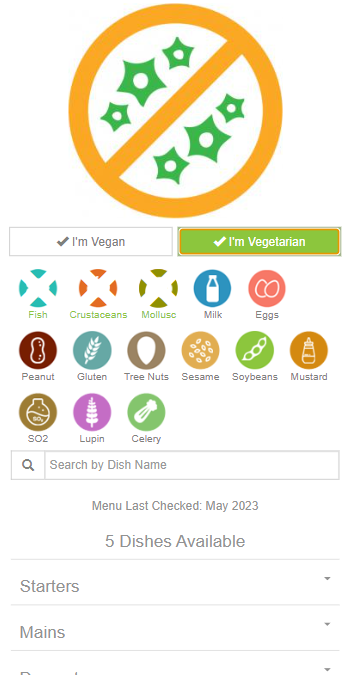
\includegraphics[width=0.62\linewidth]{master-thesis/img/allergen_menu_screenshot.png}
  \caption{The Allergy Menu application}
\end{figure}

\subsection{Tenkites}

\section{Applications for menu creation}
For restaurant employee

\section{Comparison of the applications}
\subsection{Applications with interactive menus}
% - aplikácia automaticky preloží menu do jazyka v ktorom je UI

\begin{center}
  \begin{tabular}{| l | l |}
    \hline
    1 & Allow a guest to create a dietary profile. \\
    \hline
    2 & Display a personalized menu to a guest. \\
    \hline
    3 & Allow a guest to filter out items of a menu which they cannot eat. \\
    \hline
    4 & Display a menu after a quest scans a QR code on a printed menu. \\
    \hline
    5 & Allow a guest to mark a restaurant as their favorite. \\
    \hline
    6 & The guest has control over their data. \\
    \hline
    7 & Translate a menu to the language of the UI. \\
    \hline
  \end{tabular}
  \newline
\end{center}

\begin{center}
  \begin{tabular}{| l | c | c | c |}
    \hline
      & A1 & A2 & A3 \\
    \hline
    App1 & \ding{52} & \ding{56} & \ding{115} \\
    \hline
    App2 & \ding{52} & \ding{56} & \ding{56} \\
    \hline
  \end{tabular}
  \newline
\end{center}

\subsection{Applications for menu creation}
\begin{center}
  \begin{tabular}{| l | l |}
    \hline
    1 & Automatically add allergens to an item of a menu. \\
    \hline
    2 & Allow a restaurant employee to choose whether to use allergen names or numbers in a menu. \\
    \hline
    3 & Provide templates for creating a new menu. \\
    \hline
    4 & Allow a restaurant employee to reuse a previously created menu item. \\
    \hline
    5 & The restaurant employee has control over the restaurant's data. \\
    \hline
    6 &  \\
    \hline
    7 &  \\
    \hline
  \end{tabular}
  \newline
\end{center}

\begin{center}
  \begin{tabular}{| l | c | c | c |}
    \hline
      & A1 & A2 & A3 \\
    \hline
    App1 & \ding{52} & \ding{56} & \ding{115} \\
    \hline
    App2 & \ding{52} & \ding{56} & \ding{56} \\
    \hline
  \end{tabular}
  \newline
\end{center}


\todo[inline]{add Other applications worth mentioning section}

% \section{Other applications worth mentioning}
